\documentclass{beamer} 
	% draft: Opción para que beamer no compile todos los pauses 

%%%%%%%%%%%%%%%%%%%%%%%%%%%%%%%%%%%%%%%%%%%%%%%%%%%%%%%%%%%%%%%%%%%
% CONFIGURACIÓN BEAMER                                            %
%%%%%%%%%%%%%%%%%%%%%%%%%%%%%%%%%%%%%%%%%%%%%%%%%%%%%%%%%%%%%%%%%%%

% Delete this, if you do not want the table of contents to pop up at
% the beginning of each subsection:
%\AtBeginSubsection[]
%{
%  \begin{frame}<beamer>
%    \frametitle{Contenidos}
%    \tableofcontents[currentsection,currentsubsection]
%  \end{frame}
%}

% If you wish to uncover everything in a step-wise fashion, uncomment
% the following command: 

%\beamerdefaultoverlayspecification{<+->}

\mode<presentation>
{
  \usetheme{Darmstadt} % Warsaw, Berlin, Frankfurt, Berkeley, Montpellier,Goettingen,Marburg,Hannover,Ilmenau,Dresden,Darmstadt,Singapore
     \usecolortheme{rose} %lily, rose, orchid
     \usecolortheme{whale} % seahorse, whale, albatross, dove (blanco), seagull, crane(amarillo), beetle, wolverine, dolphin
	
  \useinnertheme{rectangles}
  %\useoutertheme{split}
	\usefonttheme[onlylarge]{structuresmallcapsserif}
	\usefonttheme[onlysmall]{structurebold}
  \setbeamercovered{transparent}
	\setbeamerfont{title}{shape=\itshape,family=\rmfamily}
	%\setbeamercolor{title}{fg=black!80!white, bg=black!20!white}
  
}

\definecolor{verde}{rgb}{0,0.5,0}
\definecolor{azul}{rgb}{0,0,0.7}

\usepackage[utf8]{inputenc}
\usepackage{amsmath,amssymb,amsfonts,amsthm,amscd}
\usepackage{array}


% Entornos--------------------------------------%
\newtheorem*{definicion}{Definición}
\newtheorem*{teor}{Teorema}
\newtheorem*{prop}{Proposición}
\newtheorem*{coro}{Corolario}
\newtheorem*{defi}{Definición}
\newtheorem*{lema}{Lema}



%%%%%%%%%%%%%%%%%%%%%%%%%%%%%%%%%%%%%%%%%%%%%%%%%%%%%%%%%%%%%%%%%%%
% INFORMACIÓN DEL DOCUMENTO                                       %
%%%%%%%%%%%%%%%%%%%%%%%%%%%%%%%%%%%%%%%%%%%%%%%%%%%%%%%%%%%%%%%%%%%

\title{Ejercicio de Beamer}

\subtitle{Taller avanzado de \LaTeX}


\author{David Cabezas Berrido}

%\date{14 de marzo de 2022}

\pgfdeclareimage[height=1.2cm]{logo-titulo}{logougr}
\titlegraphic{\pgfuseimage{logo-titulo}}


%\includeonlyframes{current} % Compila sólo los frames con label=current
%Para especificar la etiqueta se escribe \begin{frame}[label=etiqueta]
%\setbeamertemplate{navigation symbols}{}
\setbeamercovered{invisible}

\begin{document}

\begin{frame}[plain]
\titlepage
\end{frame}

\begin{frame}{Indice}
\tableofcontents
\end{frame}

\section{Sección 1}

\begin{frame}{Pause: let's count in English!}
One\pause\quad Two\pause\quad Three\pause

Four\pause

\begin{itemize}
    \item Five\pause
    \item Six\pause
    \item Seven\pause
    \item Eight\pause
    \item Nine\pause
\end{itemize}
    
\begin{block}{And finally\ldots}
    Ten
\end{block}    
    
\end{frame}

\begin{frame}{Uncover: Let's count backwards}
    \uncover<10->{Ten}\quad \uncover<9->{Nine\quad} \uncover<8->{Eight}
    \uncover<7->{Seven}
\begin{itemize}
    \item \uncover<6->{Six}
    \item \uncover<5->{Five} \uncover<8->{\alert<8>{Four}}
    \item \uncover<4-7>{Four}
    \item \uncover<3->{Three}
    \item \uncover<2->{Two}
\end{itemize}
\uncover<1->{\begin{block}{First}
    One
\end{block}}
\end{frame}

\section{Sección 2}

\begin{frame}{Only+columns}
    \begin{columns}[T]
    \begin{column}{0.33\textwidth}
        \only<1-6>{
\includegraphics[width=0.8\textwidth]{beamer1}}
        \only<4->{
\includegraphics[height=3.5cm]{beamer4}}
        
        \only<7->{Seven}
    \end{column}
    
    \begin{column}{0.33\textwidth}
        \only<2-7>{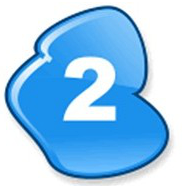
\includegraphics[width=0.8\textwidth]{beamer2}}
        \only<5-10>{
\includegraphics[height=3.5cm]{beamer5}}
        
        \only<8->{Eight}
    \end{column}
    
    \begin{column}{0.33\textwidth}
        \only<3-8>{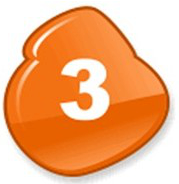
\includegraphics[width=0.8\textwidth]{beamer3}}
        \only<6-10>{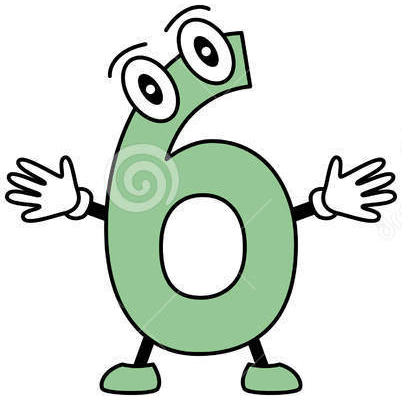
\includegraphics[height=3.5cm]{beamer6}}
        
        \only<9->{Nine}
    \end{column}
    \end{columns}
    
   \uncover<10>{ \begin{center}
    {\Huge TEN}
    \end{center}}
\end{frame}

\begin{frame}{Only+Overlayarea}
    \begin{overlayarea}{\textwidth}{2cm}
    \only<1->{
\includegraphics[height=2cm]{beamer1}}
    \only<4->{
\includegraphics[height=1.5cm]{beamer4}}
    \only<7->{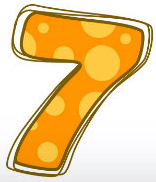
\includegraphics[height=2cm]{beamer7}}
    \end{overlayarea}
    \begin{block}{Middle numbers}<2->
    \begin{overlayarea}{\textwidth}{2cm}
    \only<2->{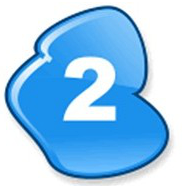
\includegraphics[height=2cm]{beamer2}}
    \only<5->{\hspace{1.5cm}
\includegraphics[height=1.5cm]{beamer5}}
    \only<8->{\hspace{2cm}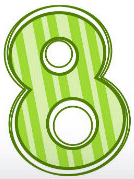
\includegraphics[height=2cm]{beamer8}}
    \end{overlayarea}
    \end{block}
    \begin{overlayarea}{\textwidth}{2cm}
    \only<3->{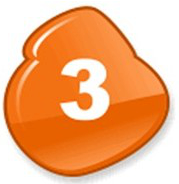
\includegraphics[height=2cm]{beamer3}}
    \only<6->{\hspace{1.5cm}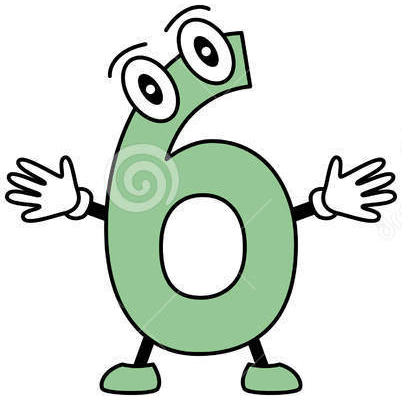
\includegraphics[height=1.5cm]{beamer6}}
    \only<9->{\hspace{3cm}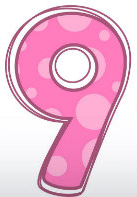
\includegraphics[height=2cm]{beamer9}}
    \end{overlayarea}
\end{frame}

\begin{frame}{Entornos matemáticos}
\begin{teor}[Pitágoras]<1-> \label{pitagoras}
Un triángulo es rectángulo si, y sólo si, uno de sus lados al cuadrado es igual a la suma de los cuadrados de los otros dos.
\end{teor}

\uncover<4->{\hyperlink{dem}{\beamerbutton{Demostración}}}

\begin{example}<3->
$3^2+4^2=5^2$
\end{example}

\begin{coro}<2->
Hay infinitos triángulos rectángulos de lados enteros.
\end{coro}
\end{frame}

\begin{frame}\label{dem}
    \begin{proof}[Demostración del teorema de Pitágoras]
    Se deja como ejercicio.
    \end{proof}
    
    \hyperlink{pitagoras}{\beamerbutton{Volver}}
\end{frame}

\begin{frame}{Entrega de ejercicios}
La evaluación de esta sesión consistirá en:
\begin{description}
   \item[80\%] Entregar este documento correctamente completado. Cambia el estilo por otro que sea de tu agrado. No adjuntes las imágenes (sólo el archivo \texttt{.tex}).
   \item[20\%] Crea una nueva diapositiva en la que incluyas una demostración completa de tu elección usando los comandos que se han visto u otros, de forma que haya un cuadro fijo \emph{overlayarea} cuyo contenido vaya cambiando.
 \end{description}
\end{frame}



\end{document}


